% !TeX root = ../report.tex
% !TeX spellcheck = en-US
% !TeX encoding = UTF-8
\chapter{DESIGN VALIDATION}\label{chap:design validation}

It is important to validate the performance of the proposed controller, this could either be done in a field test,
full-scale or scaled down, or in a virtual simulation environment. Provided that the simulated environment is an
accurate representation of the physical world. The crawler which was available at the beginning of the project was
unfortunately halfway the project, disassembled and no longer a viable method to verify the proposed controller. Roughly
around the same time, the working environment and contract of of the author changed as well. This forced validation to
be performed in a simulation. This chapter will described the simulation setup and used methods in
Section~\ref{sec:simulation}. The  results are discussed in Section~\ref{sec:results}.

\section{SIMULATION}\label{sec:simulation}
In order to tell something meaningful about performance of a controller, it has to be subject to the same physical
processes, as it would in real-life, albeit in virtual form. Section\ref{sec:motion model} lists assumed forces
and processes acting upon on a crawler and states that drive-train characteristic and soil dynamics play a huge part in
the kinematic behavior of a crawler. There are a couple of physics simulation engines that could be possible candidates
for usage in this project; These are Gazebo, Project Chrono, Bullet and PhyhsX.

From this list, only Project Chrono has an existing framework which takes into account soil dynamic behavior. This can
be simulated using a granular approach, were each particle of sand is body and is modeled using spherical rigid bodies
whose orientation is captured by Euler parameters. For each time step a complete geometric characterization of all
contacting particles is then obtained using collision detection and inter- particle normal contact forces are calculated
by allowing small inter-penetrations using a penalty method for \gls[first]{acr-DEM}. Were the normal contact force is
based on Hertz law and friction forces are calculated using the Coulomb
limit~\cite{recuero_high-fidelity_2017}\cite{serban_co-simulation_2018}. This method is computational heavy and more
suitable for detailed modeling.

An alternative method is \gls[first]{acr-SCM}, based upon the familiar Becker-Wong model. The model provides a
semi-empirical approach to the simulation of soft soil. It offers high speed of simulation and it is accurate enough for
many scenarios. It has the following attributes: it depends on few parameters (the same that are used in the Bekker-
Wong model); it can generate 3D ruts on terrains of variable height; it takes into account multi-pass hardening when
wheels generate intersecting ruts; it can work with irregular triangle-based terrain meshes; it supports an optional
refinement of the terrain mesh to capture fine details like tire threads and lugs; and, it is compatible with deformable
tires and generic shapes like obstacles, track shoes of tanks, etc. On the downside, the new soil model cannot simulate
lateral bulldozing effects like those happening when a tracked vehicle steers in-place and pushes material apart~
\cite{tasora_overview_2018}. This means that the proposed slip-prediction method can't be used in this simulation.

A big part of the physics engine, Project Chrono, is the autonomous vehicle support. This is set-up according to well
known \gls[first]{acr-OOP} practices such as, polymorphism, using virtual overrides in classes that represent physical
bodies. A custom model for different models of a drive-train, body, wheels/tracks and controller can defined and
connected as needed. Were the behavior of that individual model can be thought of as black box. As long as the interface
with the components it connects to are maintained. Section~\ref{sec:simulation model} describes the modeling of the
drive train in detail. The support of realistic sensor characteristic are not yet implemented in Project Chrono, since a
big part of the validation is measuring the performance of a Kalman Filter. An extension for Project Chrono was written,
which allows for the modeling of sensor behavior. This is extension is described in Section~\ref{sec:sensor
simulation}.

\subsection{SENSOR SIMULATION}\label{sec:sensor simulation}

% Describe the lack of sensor simulation and the need to build one

\subsection{SIMULATION MODEL}\label{sec:simulation model}

In this section a model describing the movement of a crawler is outlined. Which allows for an accurate estimate of a
predicted location and orientation of a crawler. The challenge lies in limiting uncertainties, such that path
planning algorithms can be executed without unacceptable drift of a crawler during operations.


\section{RESULTS}\label{sec:results}


\begin{RoyalFigure}[!htb, label=fig:coverage_wo_kalman]{CPP WITH/WITHOUT KALMAN FILTERING}
	\center
	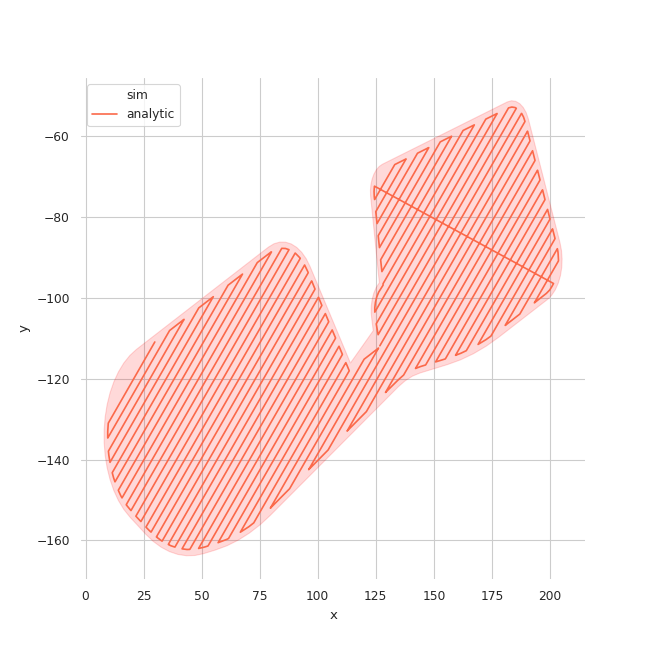
\includegraphics[width=0.333\textwidth,trim=10 10 10 10,clip]{analytic_path.png}
	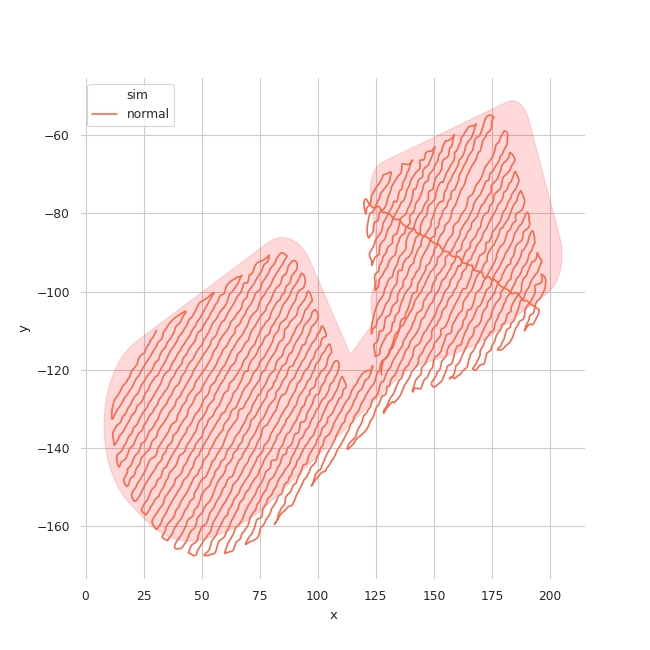
\includegraphics[width=0.333\textwidth,trim=10 10 10 10,clip]{normal_path.png}
	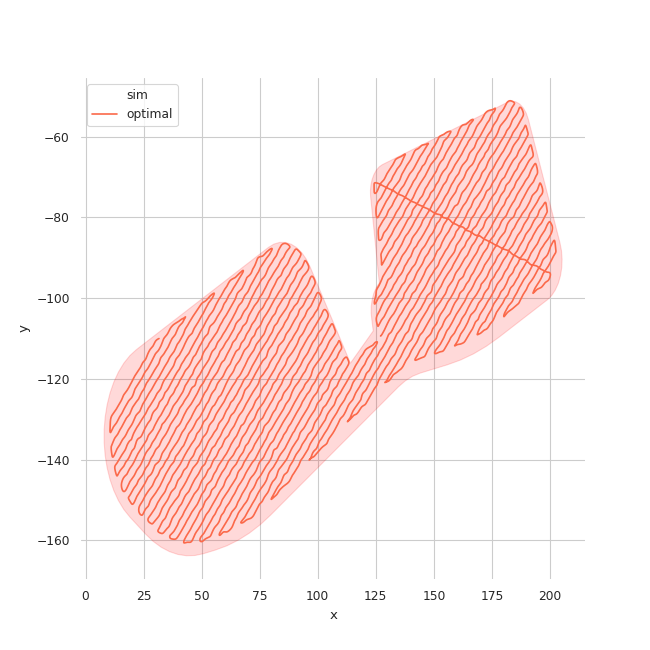
\includegraphics[width=0.333\textwidth,trim=10 10 10 10,clip]{optimal_path.png}
\end{RoyalFigure}

\begin{RoyalFigure}[!htb, label=fig:NEES_kalman]{NEES OF THE CONTROLLER}
	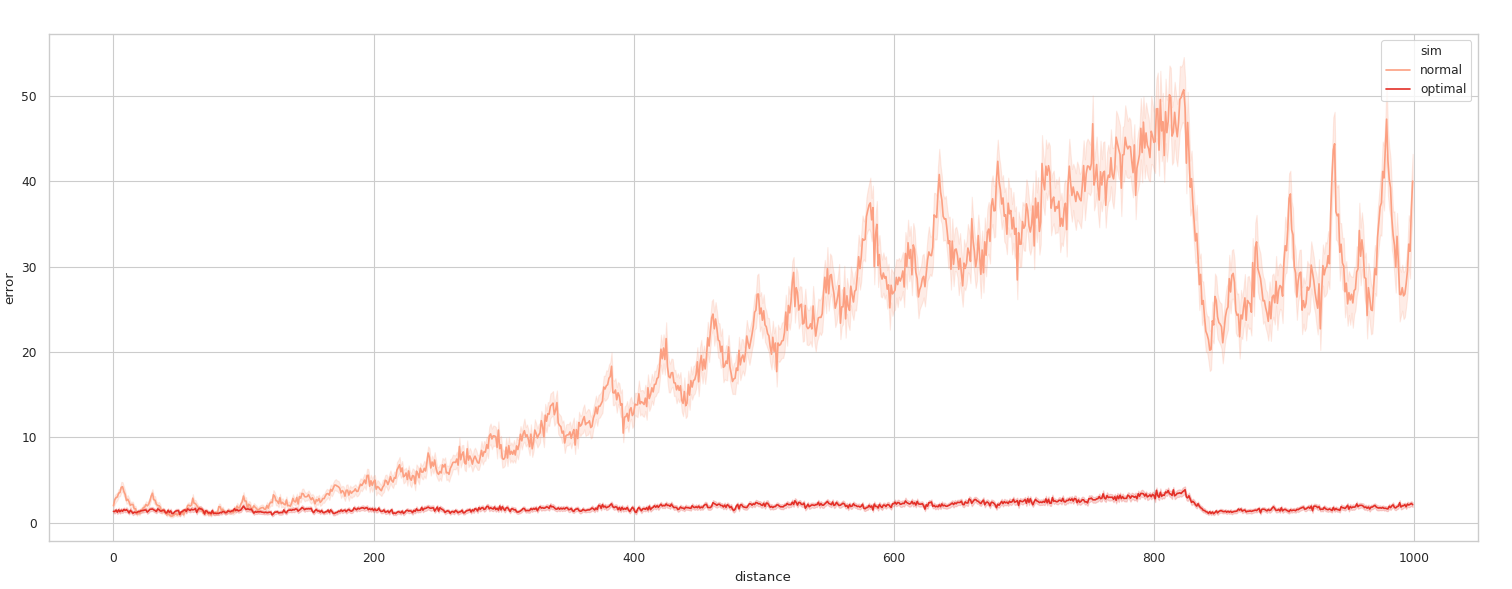
\includegraphics[width=\textwidth,trim=10 10 10 10,clip]{NEES_compared.png}
\end{RoyalFigure}
